\section{How to estimate when planning?}
\begin{itemize}
    \item Remember the three documents that have the same information but represented differently:
        \begin{itemize}
            \item The scope statement: formal definition of everything we need to do.
            \item Work breakdown structure: user friendly description of the work to be completed.
            \item Activity list: skeleton of the project.
        \end{itemize}
    
    \item Now we will learn to estimate the actitivities. 
    \item To build a project timeline we need to estimate durations of each task, add buffers, and sequence the tasks.
\end{itemize}

\subsection{Estimating the durations}
\begin{itemize}
    \item The PM needs to estimate in time each activity, as a PM you must do all the necessary research to estimate correctly, you can ask the team to estimate but it is your responsability the time you choose. Remember you are the accountable one.
    \item The PM should not take the team's opinion as the ultimate truth, the PM must do their own research and estimate conservatively.
    \item The PM can collect statistics on team members to estimate the time correctly and accurately. The idea is to base your estimation as much on data and minimally on opinion.
\end{itemize}


%%%%%%%%%%%%%%%%%%%%%%%%%%%%%%%%%%%%%%%%%%%%%%%%%%%%%%
\section{The planning fallacy, optimism bias, illusion of control}
\begin{itemize}
    \item Take into account that we are all subceptable to the planning fallacy. 
    \item The planning fallacy is the idea or notion that we plan and estimate based on optimistm and we all tend to underestimate the amount of time (and cost) it will take to complete a task. And predicions are often wrong becaus eof this.
        \begin{figure}[H]
            \centering
            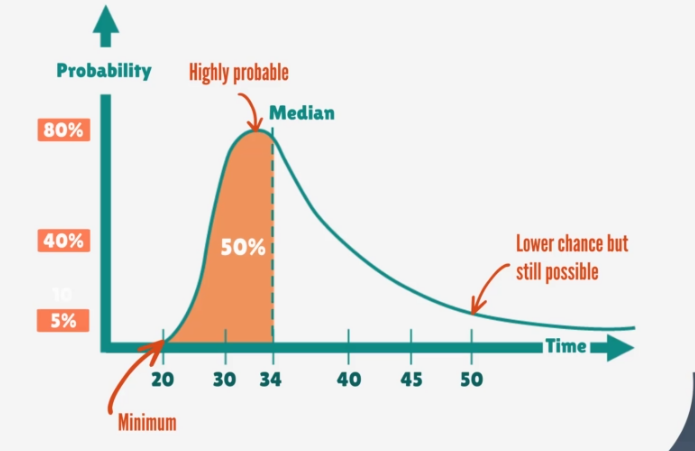
\includegraphics[width=\width\textwidth]{./figs/20221026112042.png}
            %\caption{}
        \end{figure}
    
    \item The planning fallacy was discovered by Daniel Kahneman and Amos Tversky in 1979.
    \item One of the key parts of the planning fallacy is the illusion of control, the idea that we control events. 
    \item People are generally bad at planning.
    \item As a PM you must be aware of these human biases.
    \item Estimation is a complex activity.
\end{itemize}

\subsection{The three point estimate}
\begin{itemize}
    \item When a PM is stuck and cannot estimate correcly there is a formula you can use.
    \item Identify these three components:
        \begin{enumerate}
            \item O as the optimistic time estimate.
            \item M as the most likely or normal time estimate.
            \item P the pesimistic time estimate.
        \end{enumerate}
        \[
            T = \frac{(O + 4M + P)}{6}  
        \]
    
    \item Even this has a 50\% of finishing before and 50\% chance of finishing after. This is where buffers come in.
\end{itemize}

%%%%%%%%%%%%%%%%%%%%%%%%%%%%%%%%%%%%%%%%%%%%%%%%%%%%%%
\section{How much to buffer?}
\begin{itemize}
    \item First we need to account Murphy's law:''anything that can go wrong will go wrong´´.
    \item We don't control all so the adaptation to this law is to structure the project in such a way that if the worse does happen this will cause the least amount of damage. Using plan B (B stands for buffer).
    \item When estimating a time line the PM needs to put additional time buffers that cover possible delays:
        \begin{figure}[H]
            \centering
            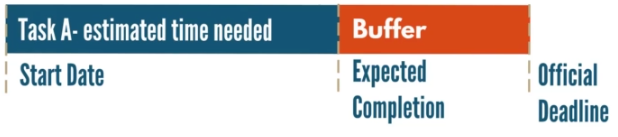
\includegraphics[width=\width\textwidth]{./figs/20221026112927.png}
            %\caption{}
        \end{figure}
    
    \item Buffer may be added to individual tasks, groups of tasks, activities or a projects.
    \item Choosing the buffer is tricky but the following guidelines are helpful.
\end{itemize}

\subsection{Buffer estimation guidelines}
\begin{enumerate}
    \item The higher the level of uncertainty the longer the buffer.
        \begin{itemize}
            \item Example.
                \begin{figure}[H]
                    \centering
                    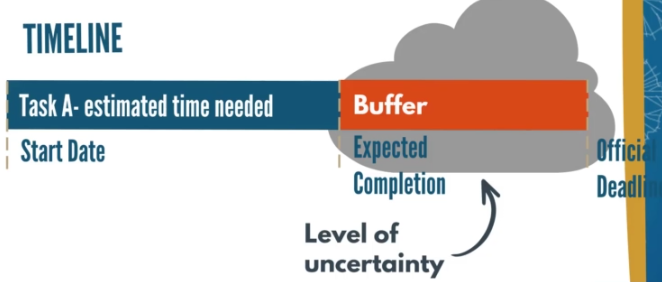
\includegraphics[width=\width\textwidth]{./figs/20221026113052.png}
                    %\caption{}
                \end{figure}
        
        \item For example if you are workign with people you have never worked before, you must take into account the possible problems that might reveal, and the buffer must reflect and cover that.
        \item The key word is accountability here.
        \end{itemize}
    \item If there is a task that will damage the project if delayed, then a longer buffer would be sensible.
        \begin{itemize}
            \item The criticality of some tasks will be higher because if delayed they delay all the others that follow them.
            \item One way to determine this is using the critical path chart (which we will see later).
        \end{itemize}
    
    \item The owner of a task is a factor:
        \begin{itemize}
            \item The experience factor plays a role. Someone with experience will be able to work better than someone without experience. Simply because there is a higher degree of uncertainty with the inexperienced.
        \end{itemize}
    
    \item Avoid having excessive buffers and distribute buffers intelligently:
        \begin{itemize}
            \item The buffers should be distributed across the project's most uncertain activities, putting all the buffers at the end for example is a bad practice and odds are you will need to decrease it because the stake holders will think its idle time.
            \item Keep in mind that presenting the buffers as buffers may lower productivity because the team thinks that once they have finished before the buffer it's ok to be idle until the next activity is required to start. A better way is to present it as a validation period or safety check.
        \end{itemize}
\end{enumerate}

%%%%%%%%%%%%%%%%%%%%%%%%%%%%%%%%%%%%%%%%%%%%%%%%%%%%%%
\section{Identifying dependencies}
\begin{itemize}
    \item By now the project should have a work breakdown structure, an activity list, and an estimated time per task along with buffers. Now we must check what activity is dependent on another. So that we can parallelize tasks that don't depend on each other.
    \item There are types of dependence outlined belowed.
\end{itemize}

\subsection{Types of dependencies}
\begin{enumerate}
    \item Logical dependency: for example you cannot install windows without having walls.
    \item Resource constraints: sometimes all though some tasks can be parallelized there just isnt enough resources to perform them at the same time. If you onnly have 1 business analysts and you need a business analysis done, you cannot expect the BA to perform this simultaneously.
    \item External constraints: activities affected by external factors such as weather. For example painting cannot be done in a rainy day.
    \item Soft dependencies: dependencies that change during program execution
\end{enumerate}

\subsection{Other types of dependencies}
\begin{enumerate}
    \item Finish to start: second task cannot start until the first task is finished (waterfall).
    \item Finish to finish: second task cannot finish until the first task has been finished.
    \item Start to start: the second task cannot start until the first starts.
    \item Start to finish: the second task has to start before the first can finish. An example is a shift of guards, the guard who is staring his shift must start before the guard who is leaving finishes his shift, this allows no windows for thiefs to break in.
\end{enumerate}

%%%%%%%%%%%%%%%%%%%%%%%%%%%%%%%%%%%%%%%%%%%%%%%%%%%%%%
\section{Identifying the critical path}
\begin{itemize}
    \item Given the completed list of activities with their buffers.
    \item So now you must identify the dependencies across the activities.
    \item Next you identify the longest chain of dependant activities as outlined in the following image:
        \begin{figure}[H]
            \centering
            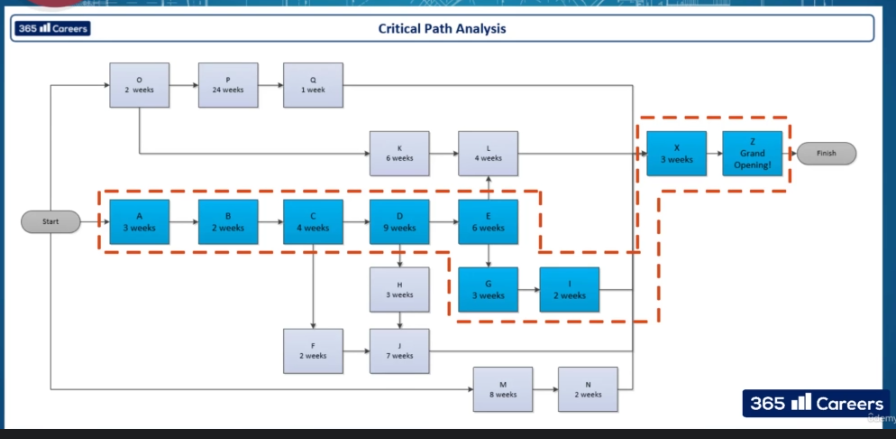
\includegraphics[width=\width\textwidth]{./figs/20221026150330.png}
            %\caption{}
        \end{figure}
    
    \item To start this use a network graph that identifies the dependencies across activities and then turn that into a critical path chart. Each box in this diagram will be a task with its duration, and each dependency will be a line connecting the dependant activity.
        \begin{figure}[H]
            \centering
            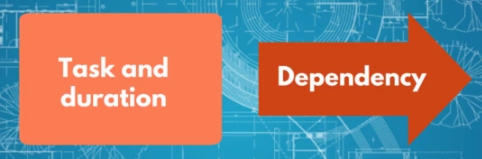
\includegraphics[width=\width\textwidth]{./figs/20221026150514.png}
            %\caption{}
        \end{figure}

    \item Given a work breakdown and the activity list.
    \item Now the longest chain of activities is the critical path, since any delay here will pospone the whole project.
        \begin{figure}[H]
            \centering
            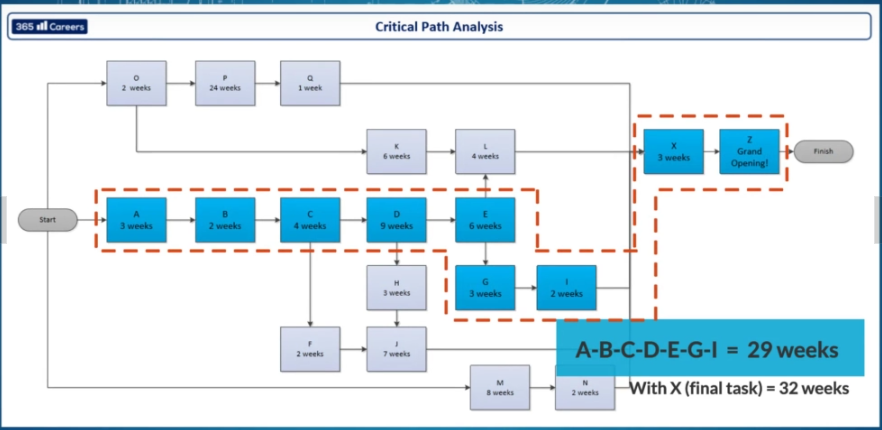
\includegraphics[width=\width\textwidth]{./figs/20221026150703.png}
            %\caption{}
        \end{figure}
    
    \item With the non-critical paths you have time, a delay most likely will not halt the whole project. This time that we are calling 'extra' is called floating time.
    \item Another very important thing to consider is that the critical path can change when there is a delay in any non critical path. If the delay is big enough and overlaps with other activities, this means that resources may become cosntrained. For example in the below image we see that originaly the middle path was the critical path but since there was a delay in a non critical task now due to that delay the new critical path will be the delayed task. This is partially why buffers are so important. 
        \begin{figure}[H]
            \centering
            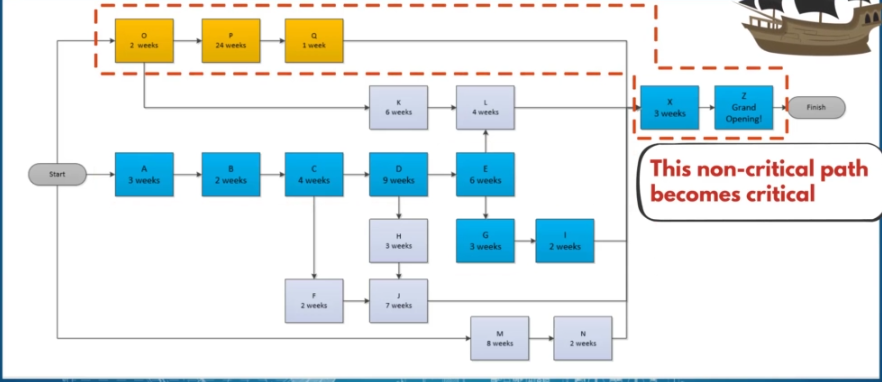
\includegraphics[width=\width\textwidth]{./figs/20221026151015.png}
            %\caption{}
        \end{figure}
    
    \item Now we may as well call the project schedule done, however there is one thing missing. The gantt chart.
\end{itemize}

%%%%%%%%%%%%%%%%%%%%%%%%%%%%%%%%%%%%%%%%%%%%%%%%%%%%%%
\section{Using the Gantt chart to plan the project work streams}
\begin{itemize}
    \item The critical path chart seems a little messy and we cannot visually tell when each activity starts and when it ends.
    \item To solve this we use the Gantt chart. It looks sort of like this:
        \begin{figure}[H]
            \centering
            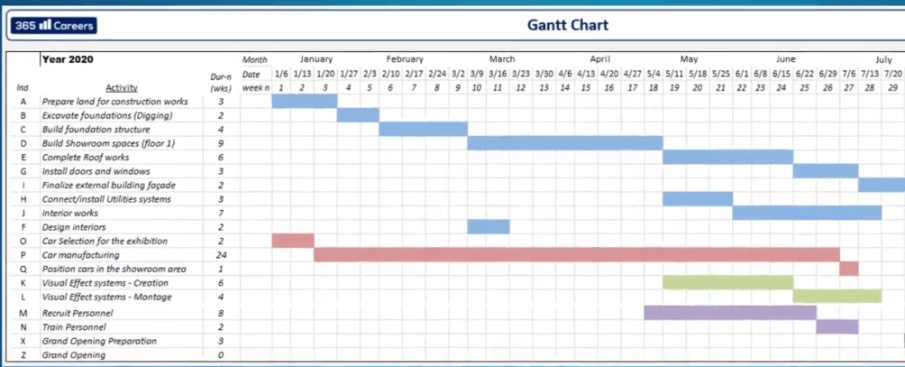
\includegraphics[width=\width\textwidth]{./figs/20221026152733.png}
            %\caption{}
        \end{figure}
    
    \item The idea is to list in the rows the activities pending and in the columns the time. Then the tasks we will parallelize will have their own space to be placed and it will be easy to see which task needs to start at end at which date. 
        \begin{figure}[H]
            \centering
            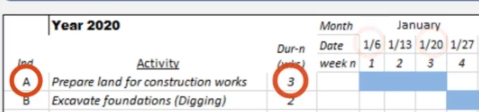
\includegraphics[width=\width\textwidth]{./figs/20221026152909.png}
            %\caption{}
        \end{figure}
    
    \item We can now visualize the duration and the start at end date clearly. Strategizing and optimizing is easier now.
\end{itemize}

%%%%%%%%%%%%%%%%%%%%%%%%%%%%%%%%%%%%%%%%%%%%%%%%%%%%%%
\section{Building the project schedule (+ MS Project tutorial)}
\begin{itemize}
    \item All of the documents seen so far (the business case, project charter, work breakdown, activity list, gantt chart) is really for this last document. Which is the master document. The project schedule document.
    \item We will be using microsoft project.
    \item It looks like this:
        \begin{figure}[H]
            \centering
            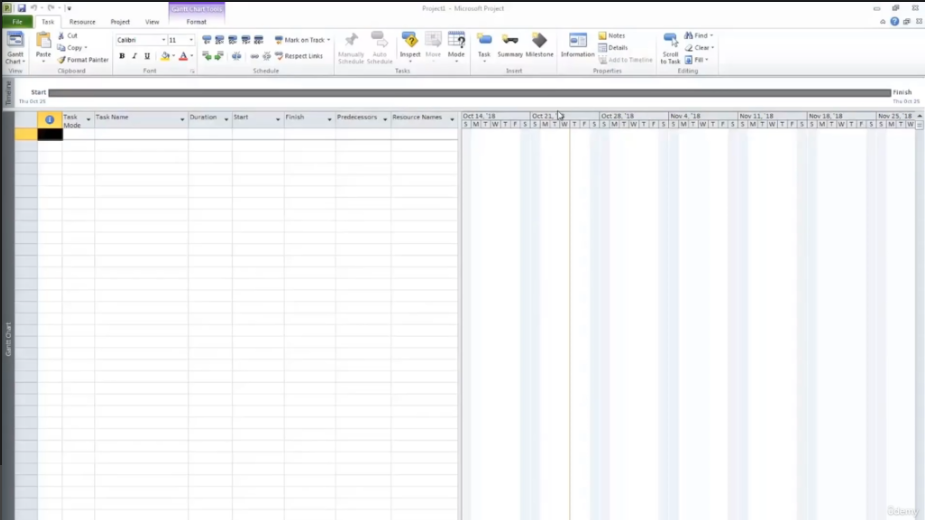
\includegraphics[width=\width\textwidth]{./figs/20221026153314.png}
            %\caption{}
        \end{figure}
        \begin{itemize}
            \item Notice the components, the left pane is for the tasks and their details and the right pane is a gantt chart that is automatically populated when you put in the dates and details.
            \item In the field predecesors is where you indicate dependencies. 
            \item Resource names is for names or roles of the person in charge of the task.
            \item To create subtasks you just need to select the tasks and indent them, this will make them subtasks to the one above.
                \begin{figure}[H]
                    \centering
                    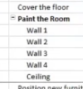
\includegraphics[width=\width\textwidth]{./figs/20221026164053.png}
                    %\caption{}
                \end{figure}
            
            \item See the automatic gantt chart of all the non-sub-tasks:
                \begin{figure}[H]
                    \centering
                    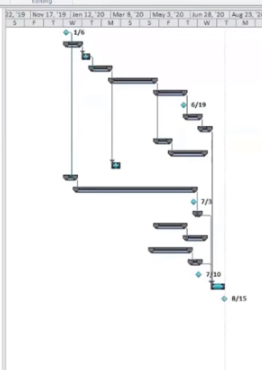
\includegraphics[width=\width\textwidth]{./figs/20221026164151.png}
                    %\caption{}
                \end{figure}
            
            \item To see the subtasks we just expand the subtasks in the left pane and this will automatically reflect the subtasks in the right pane.
        \end{itemize}
\end{itemize}

%%%%%%%%%%%%%%%%%%%%%%%%%%%%%%%%%%%%%%%%%%%%%%%%%%%%%%
\section{How to build a milestone table and its uses}
\begin{itemize}
    \item As you can imagine the ms project template can be thousands of rows and columns in extension so when any non-project manager may find this overwhelming so again we can summarize this to give the stake holders updates on the progress of the project.
    \item The milestone table document is a table that is meant to be a high level summary of the progress of the project. It includes actions, deliverables and project milestones. 
        \begin{figure}[H]
            \centering
            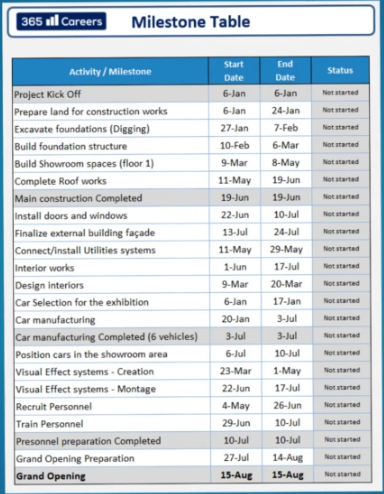
\includegraphics[width=\width\textwidth]{./figs/20221026164626.png}
            %\caption{}
        \end{figure}
    
    \item So many documents, how does this one fit in? Let's recap.
        \begin{itemize}
            \item A PM starts by creating a work breakdown structure.
            \item Then an activity list, from this list we identify the dependencies.
            \item Then the gantt chart reflects the execution of each activity and can choose which tasks aren't dependant on each other so that they can be parallelized.
            \item Then the PM will create the high-level milestone table and the low-level project plan (schedule).
        \end{itemize}
\end{itemize}